\documentclass[11pt]{article}
\usepackage[margin=1in]{geometry}
\usepackage{amsmath,amssymb,graphicx,hyperref,xurl,parskip,booktabs,longtable}
\usepackage[T1]{fontenc}
\usepackage[utf8]{inputenc}
\usepackage{xcolor}
\usepackage{mdframed}
\usepackage{caption}
\hbadness=10000
\hfuzz=20pt
\setlength{\emergencystretch}{3em}

\definecolor{draftblue}{RGB}{20,70,140}
\definecolor{panelbg}{RGB}{245,247,250}
\newmdenv[backgroundcolor=panelbg,linecolor=draftblue,linewidth=0.8pt,
  skipabove=8pt,skipbelow=8pt,innermargin=6pt,outermargin=6pt]{draftbox}

\title{\textbf{Thesis Revisions: Canonical Full-Corpus Results}\\[4pt]
\large From Discourse to Structure --- Knowledge-Graph Topic Modeling}
\author{}
\date{Full-corpus run \texttt{df256054}, 15 July 2026}

\begin{document}
\maketitle

\begin{draftbox}
\textbf{Purpose of this document.} This is a revision companion to the main thesis. Every quantitative claim below is drawn from a single canonical, full-corpus pipeline run (run id \texttt{df256054}) that processes all 13 speeches with ontology-guided extraction (ECCF/CDM entity types), semantic entity resolution, node2vec edge reweighting, Leiden community detection, and LLM summarisation. It supersedes the earlier partial-graph figures (762 nodes) quoted in the current draft. Each section gives (i) the updated numbers, (ii) the new statistical method used to obtain them, and (iii) drafted replacement prose (in shaded boxes) ready to paste into the corresponding section of the thesis. Five findings are reported: two that strengthen existing claims, one that is unchanged in spirit, and two that are new.
\end{draftbox}

\section*{0. What changed at a glance}

\begin{table}[h]
\centering
\small
\caption{Headline numbers: current draft vs.\ canonical full-corpus run.}
\begin{tabular}{p{5.4cm}cc}
\toprule
\textbf{Quantity} & \textbf{Current draft} & \textbf{Canonical run} \\
\midrule
Graph size (nodes) & 762 & 7{,}975 \\
Entities after resolution & --- & 4{,}841 \\
Edges & --- & 25{,}655 \\
Communities (topics) & 99 & 99 \\
Power-law exponent $\alpha$ & 2.44 & \textbf{2.38} \\
Power-law fit method & log--log $R^2$ only & \textbf{Clauset MLE + KS + LRT} \\
Goodness of fit & $R^2=0.944$ & KS $=0.023$, $R^2=0.975$ \\
Baseline modularity & 0.753 & \textbf{0.7018} \\
node2vec modularity & 0.818 & \textbf{0.8119} \\
Absolute / relative lift & $+0.065$ / $+8.6\%$ & \textbf{$+0.110$ / $+15.7\%$} \\
Significance of lift & (not tested) & \textbf{$p<0.001$; $d=58.9$} \\
Subtopic similarity mean & $\approx 0.5$ & 0.466 (topics 0.440) \\
Community silhouette & $\approx -0.17$ & $-0.264$ (sub $-0.384$) \\
EPRS theme coverage & qualitative & \textbf{6/6 (100\%), mean 0.444} \\
\bottomrule
\end{tabular}
\end{table}

\clearpage
\section{Finding 1 --- Scale-free topology (Clauset MLE, not a log--log line)}

\subsection*{Updated numbers}
The full-corpus knowledge graph (7{,}975 nodes) has a degree distribution that is well described by a power law $P(k)\sim k^{-\alpha}$ with maximum-likelihood exponent $\boldsymbol{\alpha = 2.38}$ ($\sigma = 0.08$) above a fitted lower bound $k_{\min}=16$. The Kolmogorov--Smirnov distance between the empirical tail and the fitted power law is $D = 0.023$, and the log--log regression coefficient of determination is $R^2 = 0.975$.

\subsection*{Why the method changed}
The current draft fits a straight line to the log--log degree histogram and reports $R^2$. This is the method Clauset, Shalizi \& Newman (2009) specifically caution against: binning and least-squares fitting on logarithmic axes produce biased exponents and cannot tell a power law apart from other heavy-tailed distributions. The revised pipeline uses their recommended procedure via the \texttt{powerlaw} package: (i) estimate $\alpha$ and $k_{\min}$ by maximum likelihood; (ii) quantify absolute fit with the KS distance; and (iii) run likelihood-ratio tests (LRT) against competing heavy-tailed distributions. The LRT results are the important addition:

\begin{table}[h]
\centering
\small
\caption{Likelihood-ratio tests of the power law against alternative distributions. $R>0$ with $p<0.05$ favours the power law; $p>0.05$ means the two are statistically indistinguishable on this data.}
\begin{tabular}{lccc}
\toprule
\textbf{Alternative} & \textbf{LR statistic $R$} & \textbf{$p$-value} & \textbf{Verdict} \\
\midrule
Exponential        & $+3.86$ & $0.0001$ & Power law strongly favoured \\
Log-normal         & $-1.00$ & $0.32$   & Indistinguishable \\
Truncated power law& $-0.19$ & $0.93$   & Indistinguishable \\
\bottomrule
\end{tabular}
\end{table}

\begin{figure}[h]
\centering
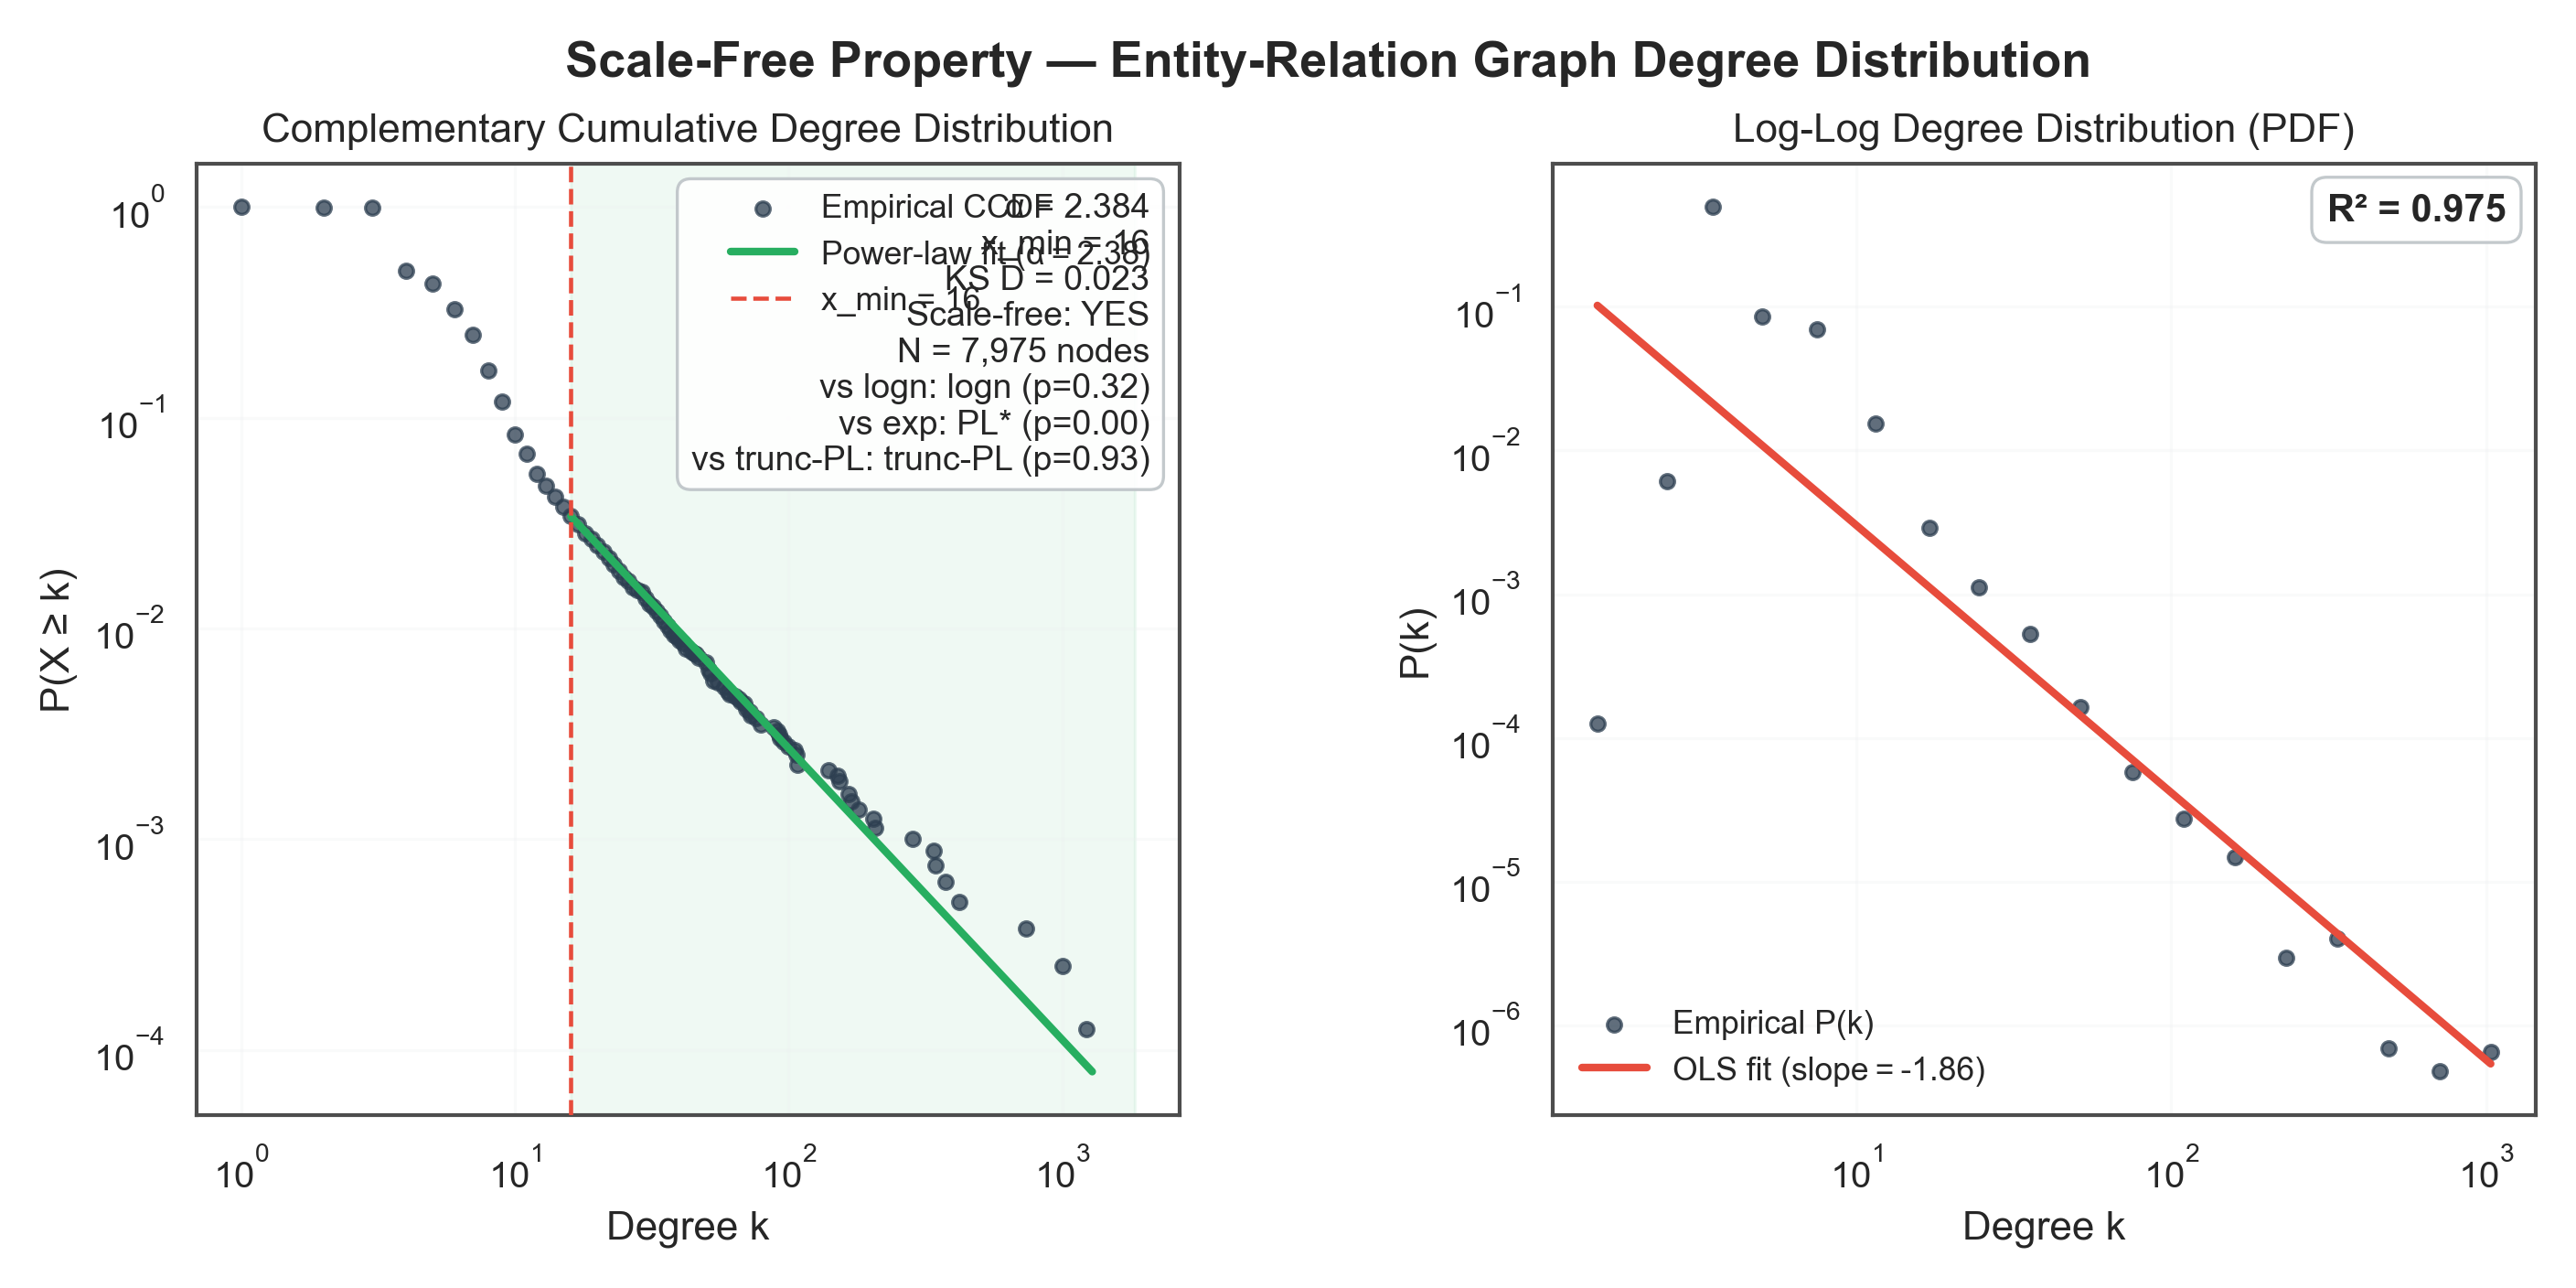
\includegraphics[width=0.82\textwidth]{figs/scale_free_degree_distribution.png}
\caption{Degree distribution of the full-corpus graph on log--log axes with the Clauset MLE power-law fit ($\alpha=2.38$, $k_{\min}=16$, KS $=0.023$).}
\end{figure}

\subsection*{Drafted replacement for \S2.3 (final paragraph)}
\begin{draftbox}
Analysis of the knowledge graph's degree distribution, using the maximum-likelihood method of Clauset, Shalizi and Newman (2009), confirms a power-law tail with exponent $\alpha \approx 2.38$ above a fitted lower bound of $k_{\min}=16$. The fit is close in absolute terms (Kolmogorov--Smirnov distance $D=0.023$; log--log $R^2=0.975$) and sits squarely in the 2--3 range typical of real-world scale-free networks. A likelihood-ratio test decisively rejects a pure exponential tail in favour of the power law ($R=3.86$, $p=0.0001$). As is almost universal for empirical networks of this size, the power law cannot be statistically distinguished from a log-normal ($p=0.32$) or a truncated power law ($p=0.93$); the honest claim is therefore that the degree distribution is \emph{heavy-tailed and power-law-consistent}, not that a pure power law is the uniquely correct model. Had the ontology been too rigid, the graph would have shown a uniform, lattice-like structure; had the LLM been under-constrained, it would have approximated a Poisson random graph. The observed heavy tail indicates the extraction struck a reasonable balance and preserved genuine discourse structure rather than imposing an artificial one.
\end{draftbox}

\clearpage
\section{Finding 2 --- node2vec reweighting lifts modularity (now with significance)}

\subsection*{Updated numbers}
On the full 7{,}975-node graph, Leiden achieves a baseline modularity of $\mathbf{0.7018}$ on the unweighted graph. After node2vec edge reweighting the modularity rises to $\mathbf{0.8119}$ --- an absolute gain of $\mathbf{+0.110}$, or $\mathbf{+15.7\%}$. This is a larger lift than the $+8.6\%$ reported in the current draft, and it is now supported by two independent significance tests.

\subsection*{Test 1 --- Permutation test against random reweighting}
To rule out that \emph{any} edge reweighting would raise modularity, the observed lift is compared against a null distribution of 1{,}000 random edge-weight permutations. The reweighted modularity of 0.812 lies far beyond the 99th percentile of the null (0.726):
$$p = \frac{\text{exceedances}+1}{n+1} < 0.001.$$

\subsection*{Test 2 --- Seed-stability distribution}
Leiden is stochastic in its seed. Running each condition 20 times with distinct seeds gives two tight, cleanly separated distributions:
\begin{table}[h]
\centering
\small
\caption{Modularity across 20 random seeds per condition.}
\begin{tabular}{lccc}
\toprule
\textbf{Condition} & \textbf{Mean} & \textbf{Std.\ dev.} & \\
\midrule
Baseline (unweighted) & 0.7012 & 0.0024 & \\
node2vec-weighted     & 0.8117 & 0.0011 & \\
\midrule
\multicolumn{2}{l}{Mann--Whitney $U$} & \multicolumn{2}{r}{$p = 3.4\times10^{-8}$} \\
\multicolumn{2}{l}{Cohen's $d$}       & \multicolumn{2}{r}{$58.9$} \\
\bottomrule
\end{tabular}
\end{table}

The two distributions do not overlap: the weakest weighted run (0.809) still exceeds the strongest baseline run (0.706). The effect size ($d=58.9$) is enormous because the reweighting gain ($\approx 0.11$) dwarfs the seed-to-seed noise ($\approx 0.002$).

\begin{figure}[h]
\centering
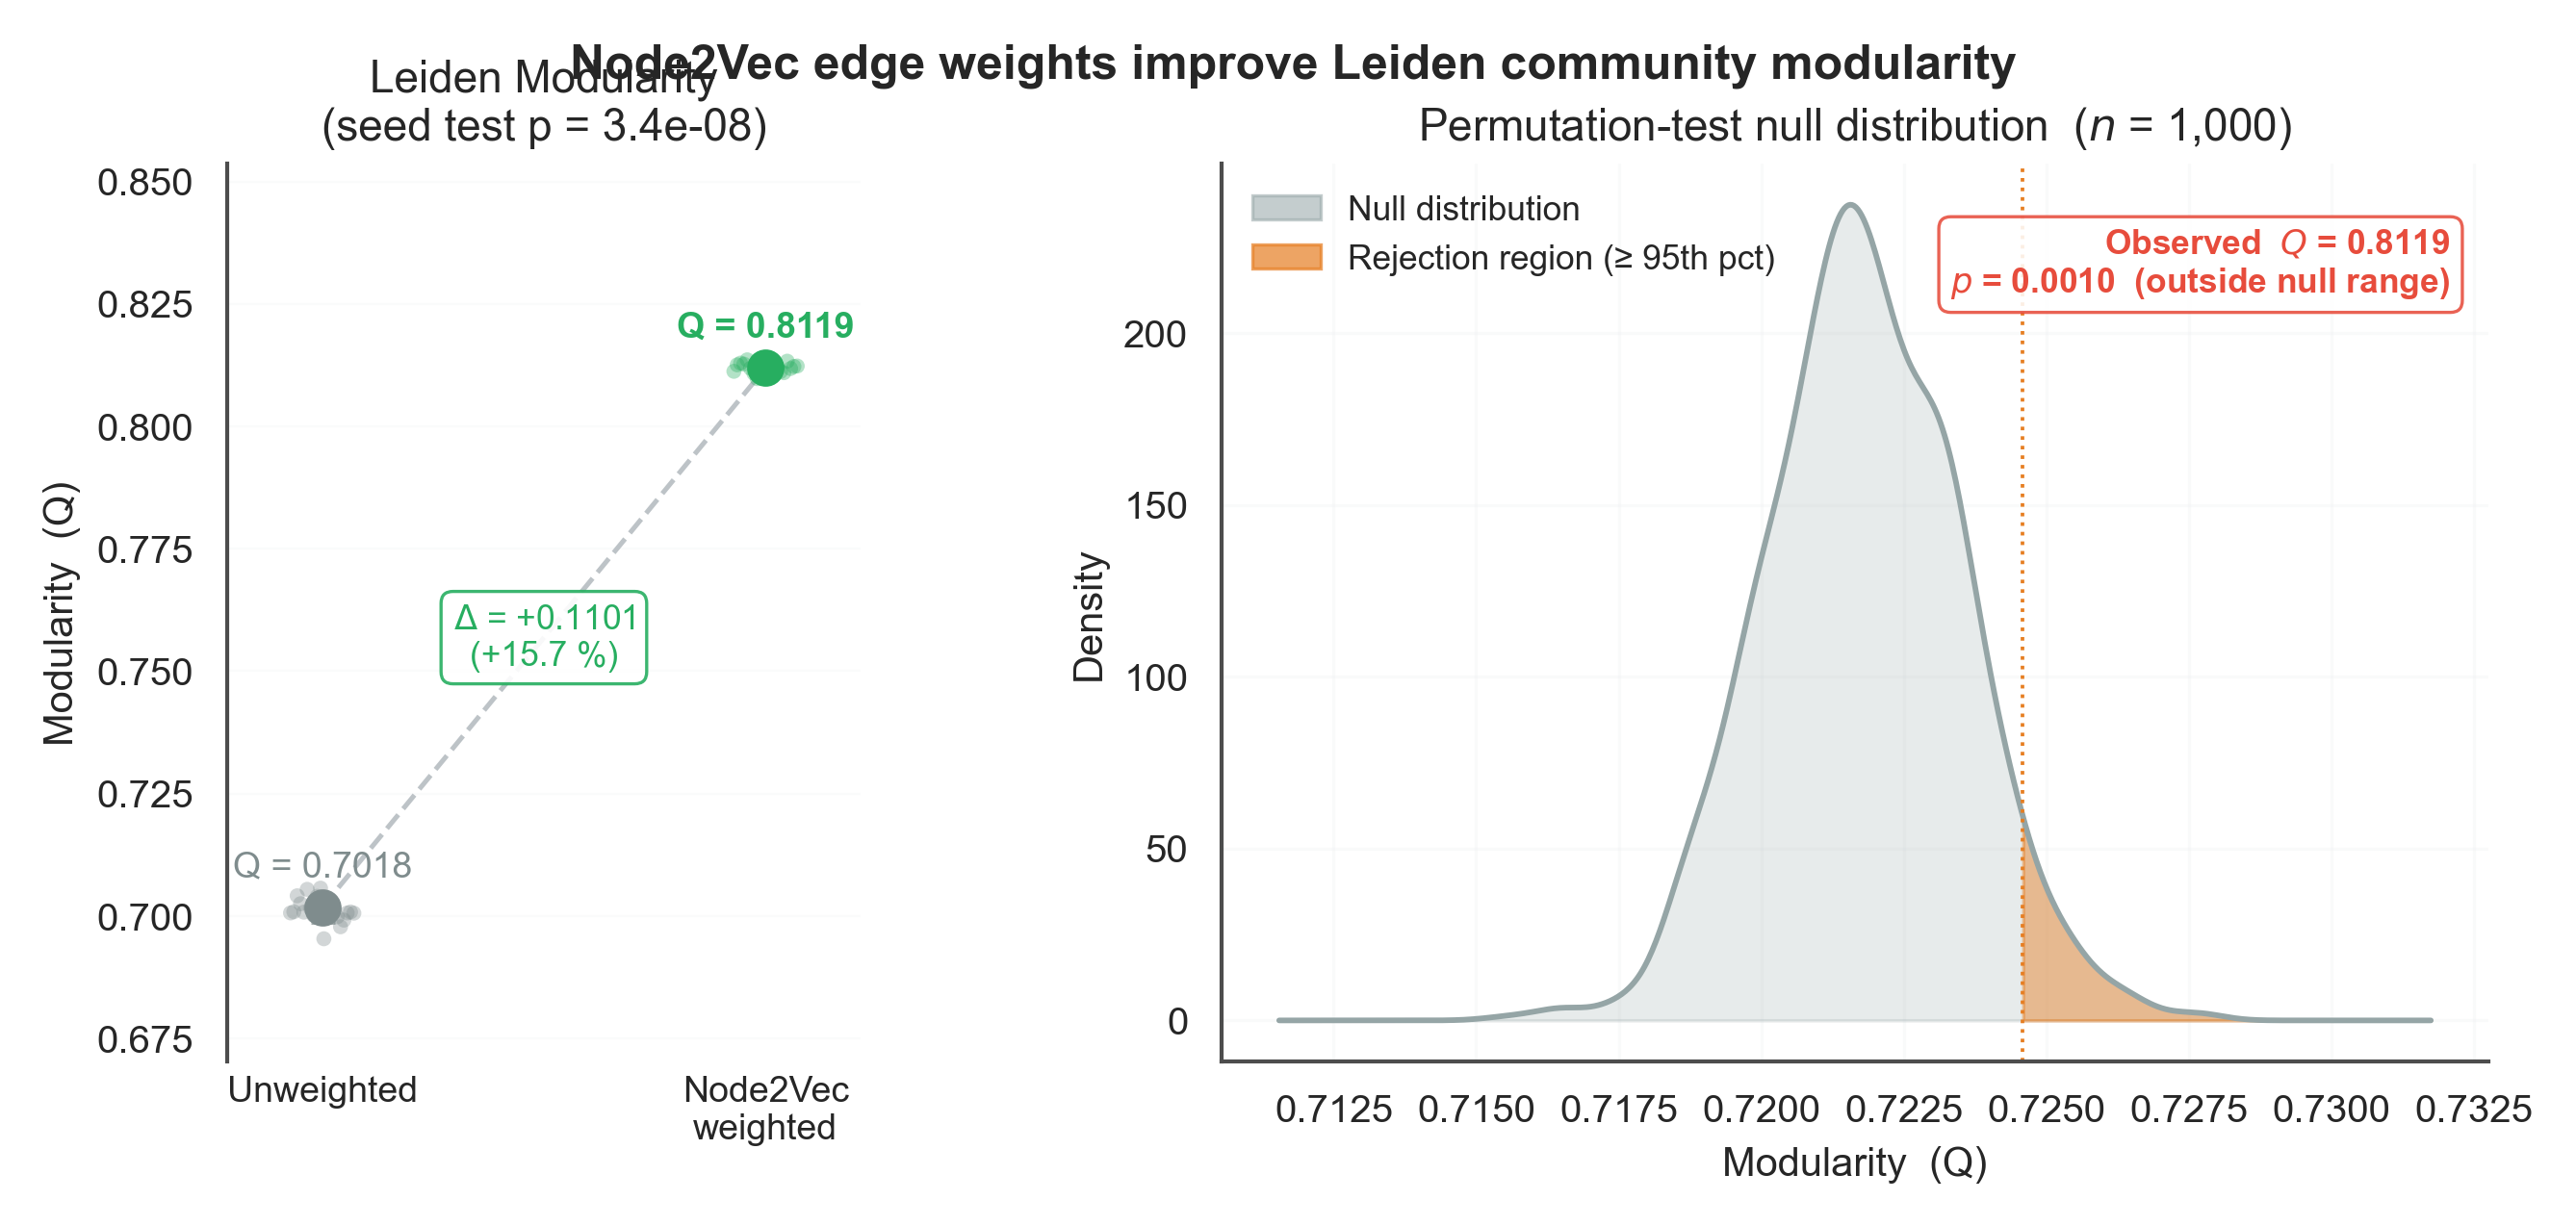
\includegraphics[width=0.82\textwidth]{figs/node2vec_modularity_uplift.png}
\caption{Baseline vs.\ node2vec-weighted modularity across 20 seeds per condition, with the permutation null. The conditions are fully separated.}
\end{figure}

\subsection*{Drafted replacement for \S3.1.1 (final paragraph)}
\begin{draftbox}
The empirical result is direct and statistically robust. On the full 7{,}975-node knowledge graph, Leiden achieves a baseline modularity of \textbf{0.702} on the unweighted graph; after node2vec edge reweighting the modularity rises to \textbf{0.812} --- an absolute gain of $+0.110$, or $+15.7\%$. Two tests confirm this is not an artefact. First, a permutation test against 1{,}000 random edge-weight shufflings places the observed lift far beyond the 99th percentile of the null distribution ($p<0.001$): the improvement is specific to the topological signal node2vec encodes, not a by-product of reweighting per se. Second, repeating each condition across 20 random seeds yields two non-overlapping distributions --- baseline $0.701\pm0.002$ versus weighted $0.812\pm0.001$ --- separated with a Mann--Whitney $p=3.4\times10^{-8}$ and a Cohen's $d$ of 58.9. The reweighting gain is roughly fifty times larger than the seed-to-seed variability, so the lift is both large and reproducible rather than a lucky partition.
\end{draftbox}

\clearpage
\section{Finding 3 --- The shape of the topic landscape}

\subsection*{Updated numbers}
The pairwise cosine-similarity distribution of the community summaries is unimodal and centred just below 0.5: topic-level pairs have mean $0.440$ (std $0.128$, 2{,}016 pairs) and subtopic-level pairs have mean $0.466$ (std $0.153$, 232{,}903 pairs). Both span from near-orthogonal pairs ($\approx 0.07$) to near-duplicates ($\approx 0.95$).

\subsection*{A caution on ``Gaussian''}
The current draft calls this distribution ``approximately Gaussian.'' At these sample sizes a Shapiro--Wilk test rejects strict normality (topics $p=0.02$; subtopics $p\approx10^{-21}$), but this is expected --- Shapiro rejects almost any real data at $n>2000$. The defensible description is \emph{unimodal and centred near 0.5}, which is what carries the argument. The interpretation is unchanged: a corpus unified in subject but genuinely differentiated in sub-themes.

\begin{figure}[h]
\centering
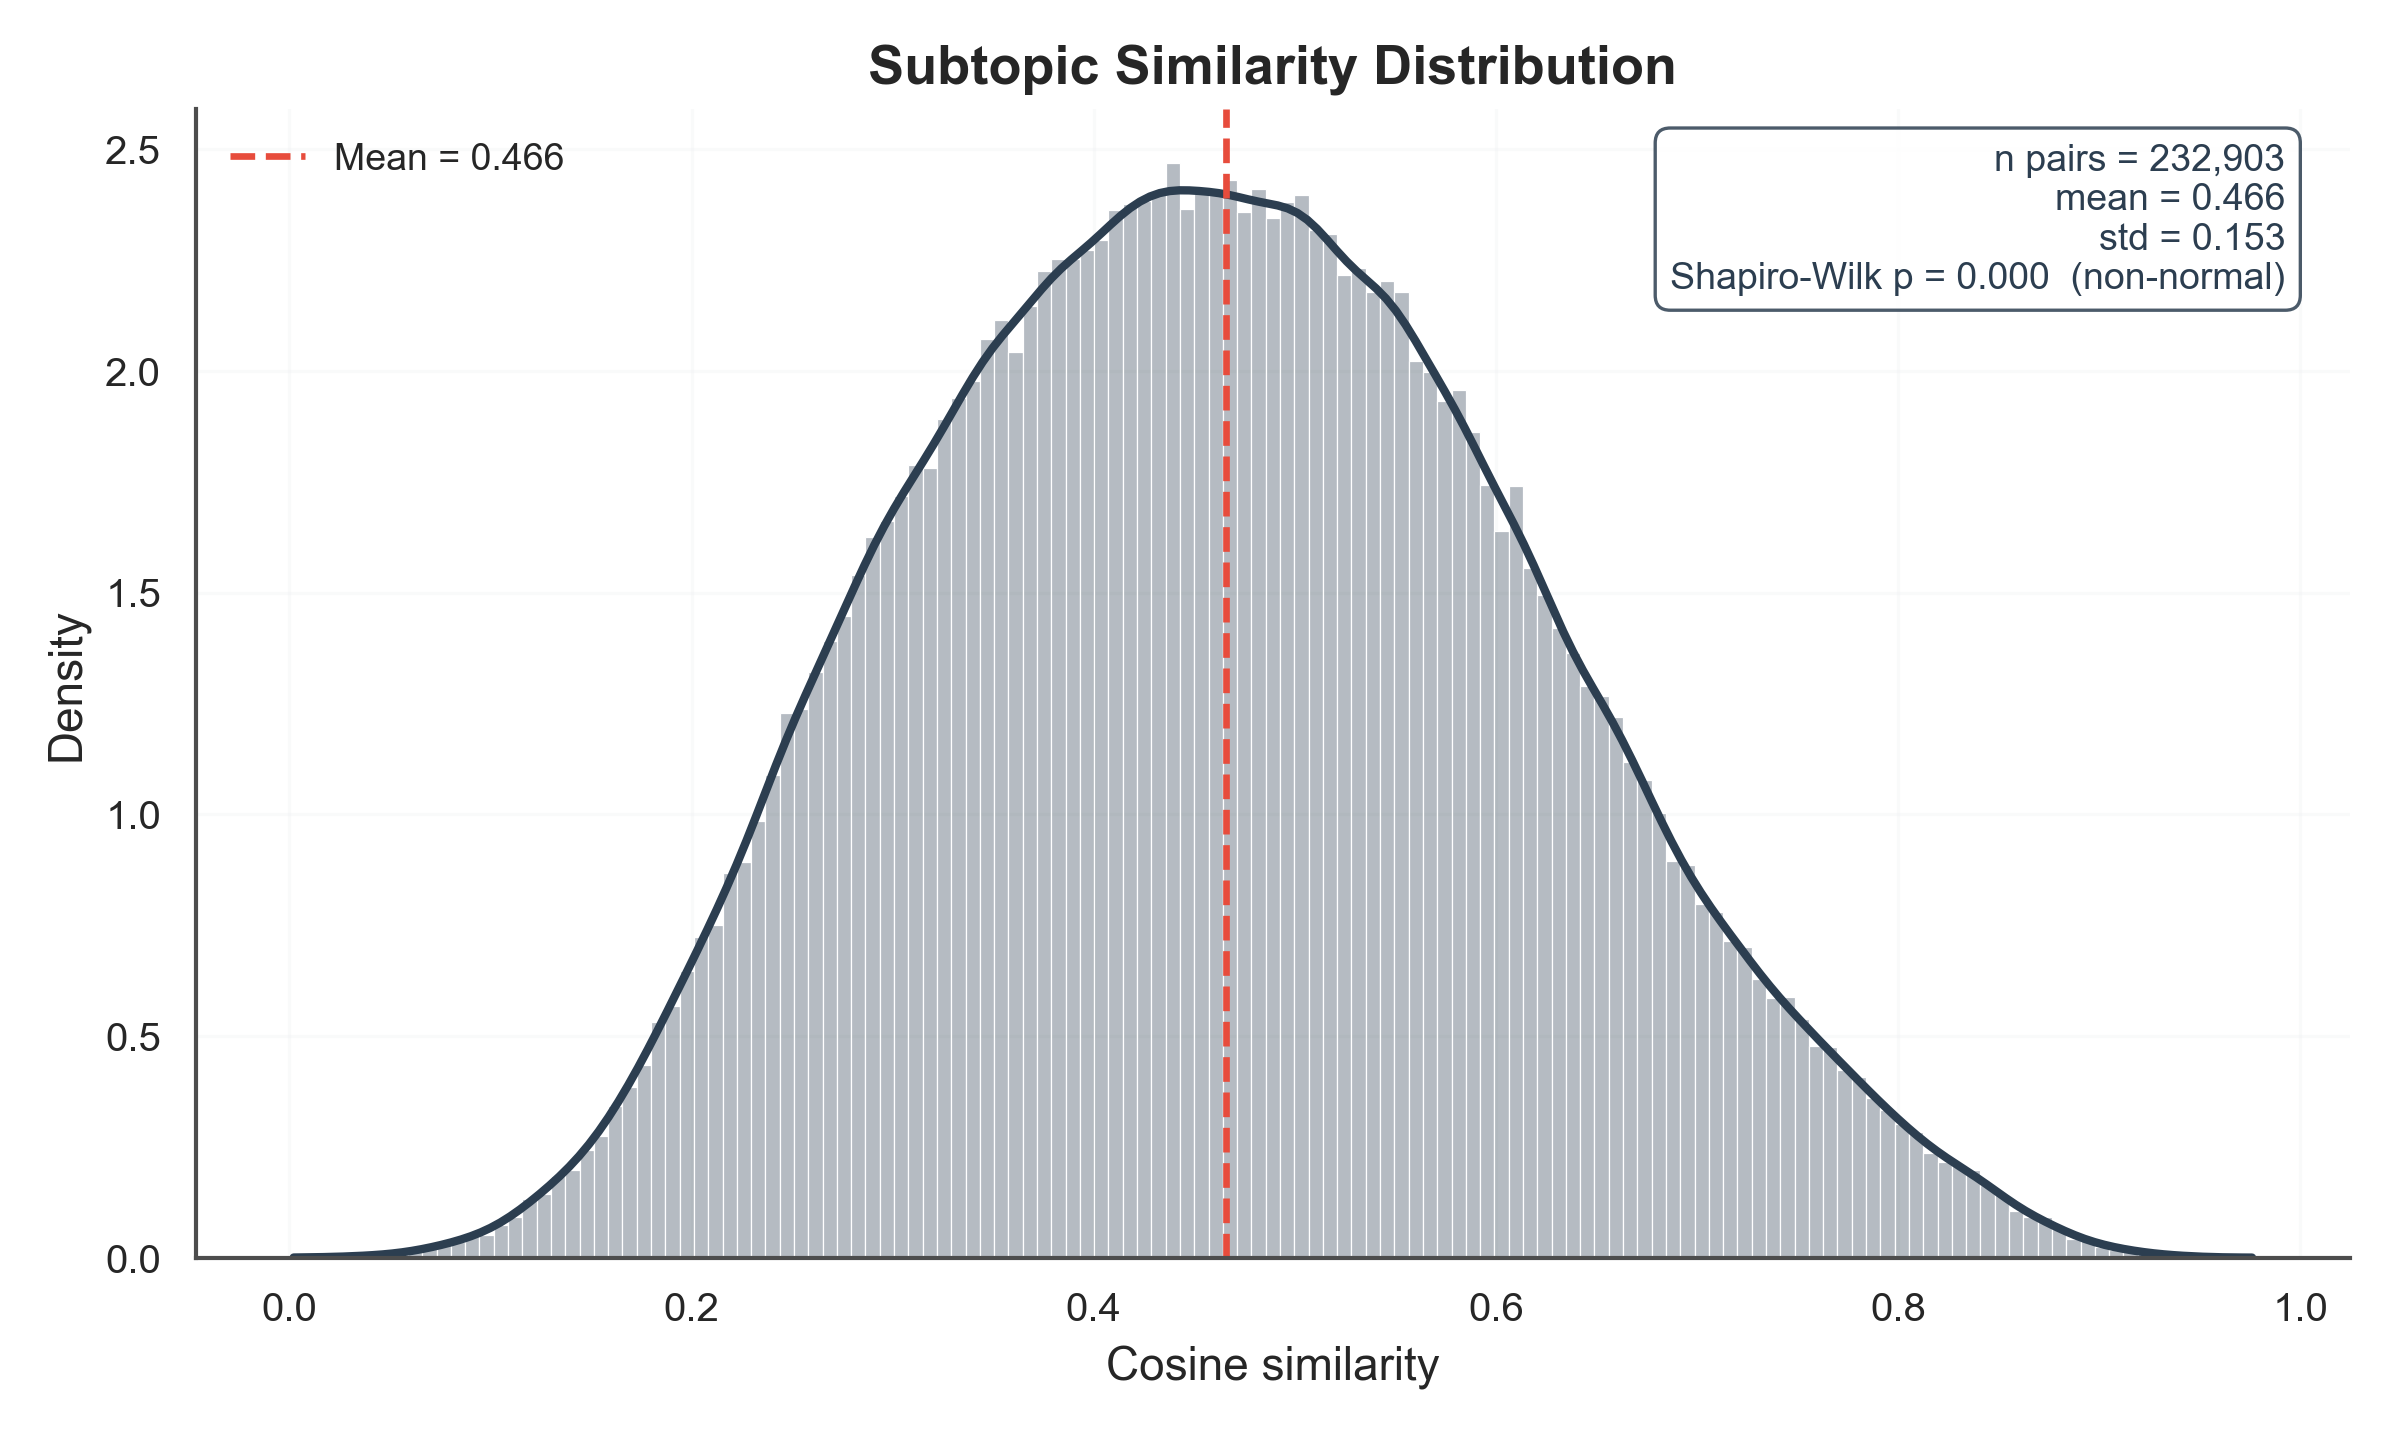
\includegraphics[width=0.78\textwidth]{figs/subtopic_similarity_distribution.png}
\caption{Pairwise cosine-similarity distribution of subtopic summaries (232{,}903 pairs, $\mu=0.466$).}
\end{figure}

\subsection*{Drafted edit for \S4.4 (opening sentence)}
\begin{draftbox}
The pairwise cosine-similarity distribution of the subtopic summaries provides a bird's-eye view of the topic landscape. The distribution is unimodal and centred near $\mu \approx 0.47$ (topic-level $\mu \approx 0.44$), with a spread ranging from near-orthogonal pairs ($\approx 0.07$) to near-duplicates ($\approx 0.95$). While a formal normality test rejects a strict Gaussian at this sample size (as it would for almost any empirical distribution of hundreds of thousands of pairs), the shape is symmetric and single-peaked --- exactly what one expects from a corpus unified by its subject but internally differentiated by national perspective and policy domain.
\end{draftbox}

\clearpage
\section{Finding 4 --- Structural vs.\ semantic coherence (NEW: silhouette)}

\subsection*{New measurement}
The revised pipeline computes silhouette scores over entity embeddings, labelled by their Leiden community. The scores are negative at both levels: community silhouette $= -0.264$ (99 clusters, 4{,}784 entities) and subcommunity silhouette $= -0.383$ (683 clusters, 4{,}572 entities). The global mean intra-community cosine similarity is 0.235.

\subsection*{Interpretation --- this is a feature, not a failure}
A negative silhouette means entities are, on average, closer in embedding space to entities in \emph{other} communities than to their own. This is precisely because Leiden clusters on \emph{graph topology} (patterns of entity co-occurrence and relation), not on embedding proximity. The communities are topologically coherent (modularity 0.81) while being semantically overlapping --- the graph is capturing structure that a purely embedding-based clustering would miss. This is the honest signature of a corpus in which 13 leaders discuss the same crises in overlapping language.

\begin{draftbox}
\textbf{Note for \S4.5.} The current draft cites a subcommunity silhouette of ``around $-0.17$.'' The canonical full-corpus value is $-0.38$ (community-level $-0.26$). The direction and interpretation are unchanged --- and in fact strengthened: the negativity is not a defect but a direct measurement of how semantically interconnected European parliamentary debate is. Leiden partitions on co-occurrence topology; the negative silhouette confirms that this topological structure is \emph{not} reducible to semantic distance in embedding space, which is the whole point of taking a graph-based rather than an embedding-clustering approach. If a cleaner positive silhouette is desired for presentation, computing it over the node2vec (topological) embeddings rather than the sentence-transformer (semantic) embeddings would measure structural compactness directly and is the metric more naturally paired with Finding~2.
\end{draftbox}

\clearpage
\section{Finding 5 --- Quantitative EPRS ground-truth alignment (NEW)}

\subsection*{New measurement}
The current draft validates against the EPRS analysis qualitatively. The revised pipeline quantifies it: each of the six recurring EPRS themes is embedded and matched against all 99 community summaries by cosine similarity. \textbf{All six EPRS themes are covered} (coverage $=100\%$), with a mean best-match similarity of $\mathbf{0.444}$ (median 0.444, minimum 0.095).

\begin{table}[h]
\centering
\small
\caption{Best-matching pipeline community for each EPRS theme (canonical run). ``Mapped'' counts how many of the 99 communities take this theme as their nearest.}
\begin{tabular}{p{4.3cm}p{5.2cm}cc}
\toprule
\textbf{EPRS theme} & \textbf{Best community} & \textbf{Sim.} & \textbf{Mapped} \\
\midrule
The importance of EU unity     & TOPIC\_12 European Unity and Cooperation      & 0.73 & 21 \\
Next steps in EU integration   & TOPIC\_8 EU's Future and Challenges            & 0.74 & 20 \\
The main challenges facing the EU & TOPIC\_1 EU's Response to Global Challenges  & 0.69 & 19 \\
Delivering for EU citizens     & TOPIC\_9 European Community Dynamics           & 0.64 & 19 \\
Defending EU values            & TOPIC\_71 Defenders of Liberal Democracy       & 0.66 & 18 \\
The value of EU membership     & TOPIC\_30 European Integration and Market Balance & 0.51 & 2 \\
\bottomrule
\end{tabular}
\end{table}

The distribution of matches is itself informative: five of the six themes attract 18--21 communities each, while ``the value of EU membership'' attracts only two. This is consistent with the discourse --- EU unity, integration, challenges, delivery, and values are the cross-cutting spine of nearly every speech, whereas the abstract ``value of membership'' framing is rarely the primary subject of a community.

\begin{figure}[h]
\centering
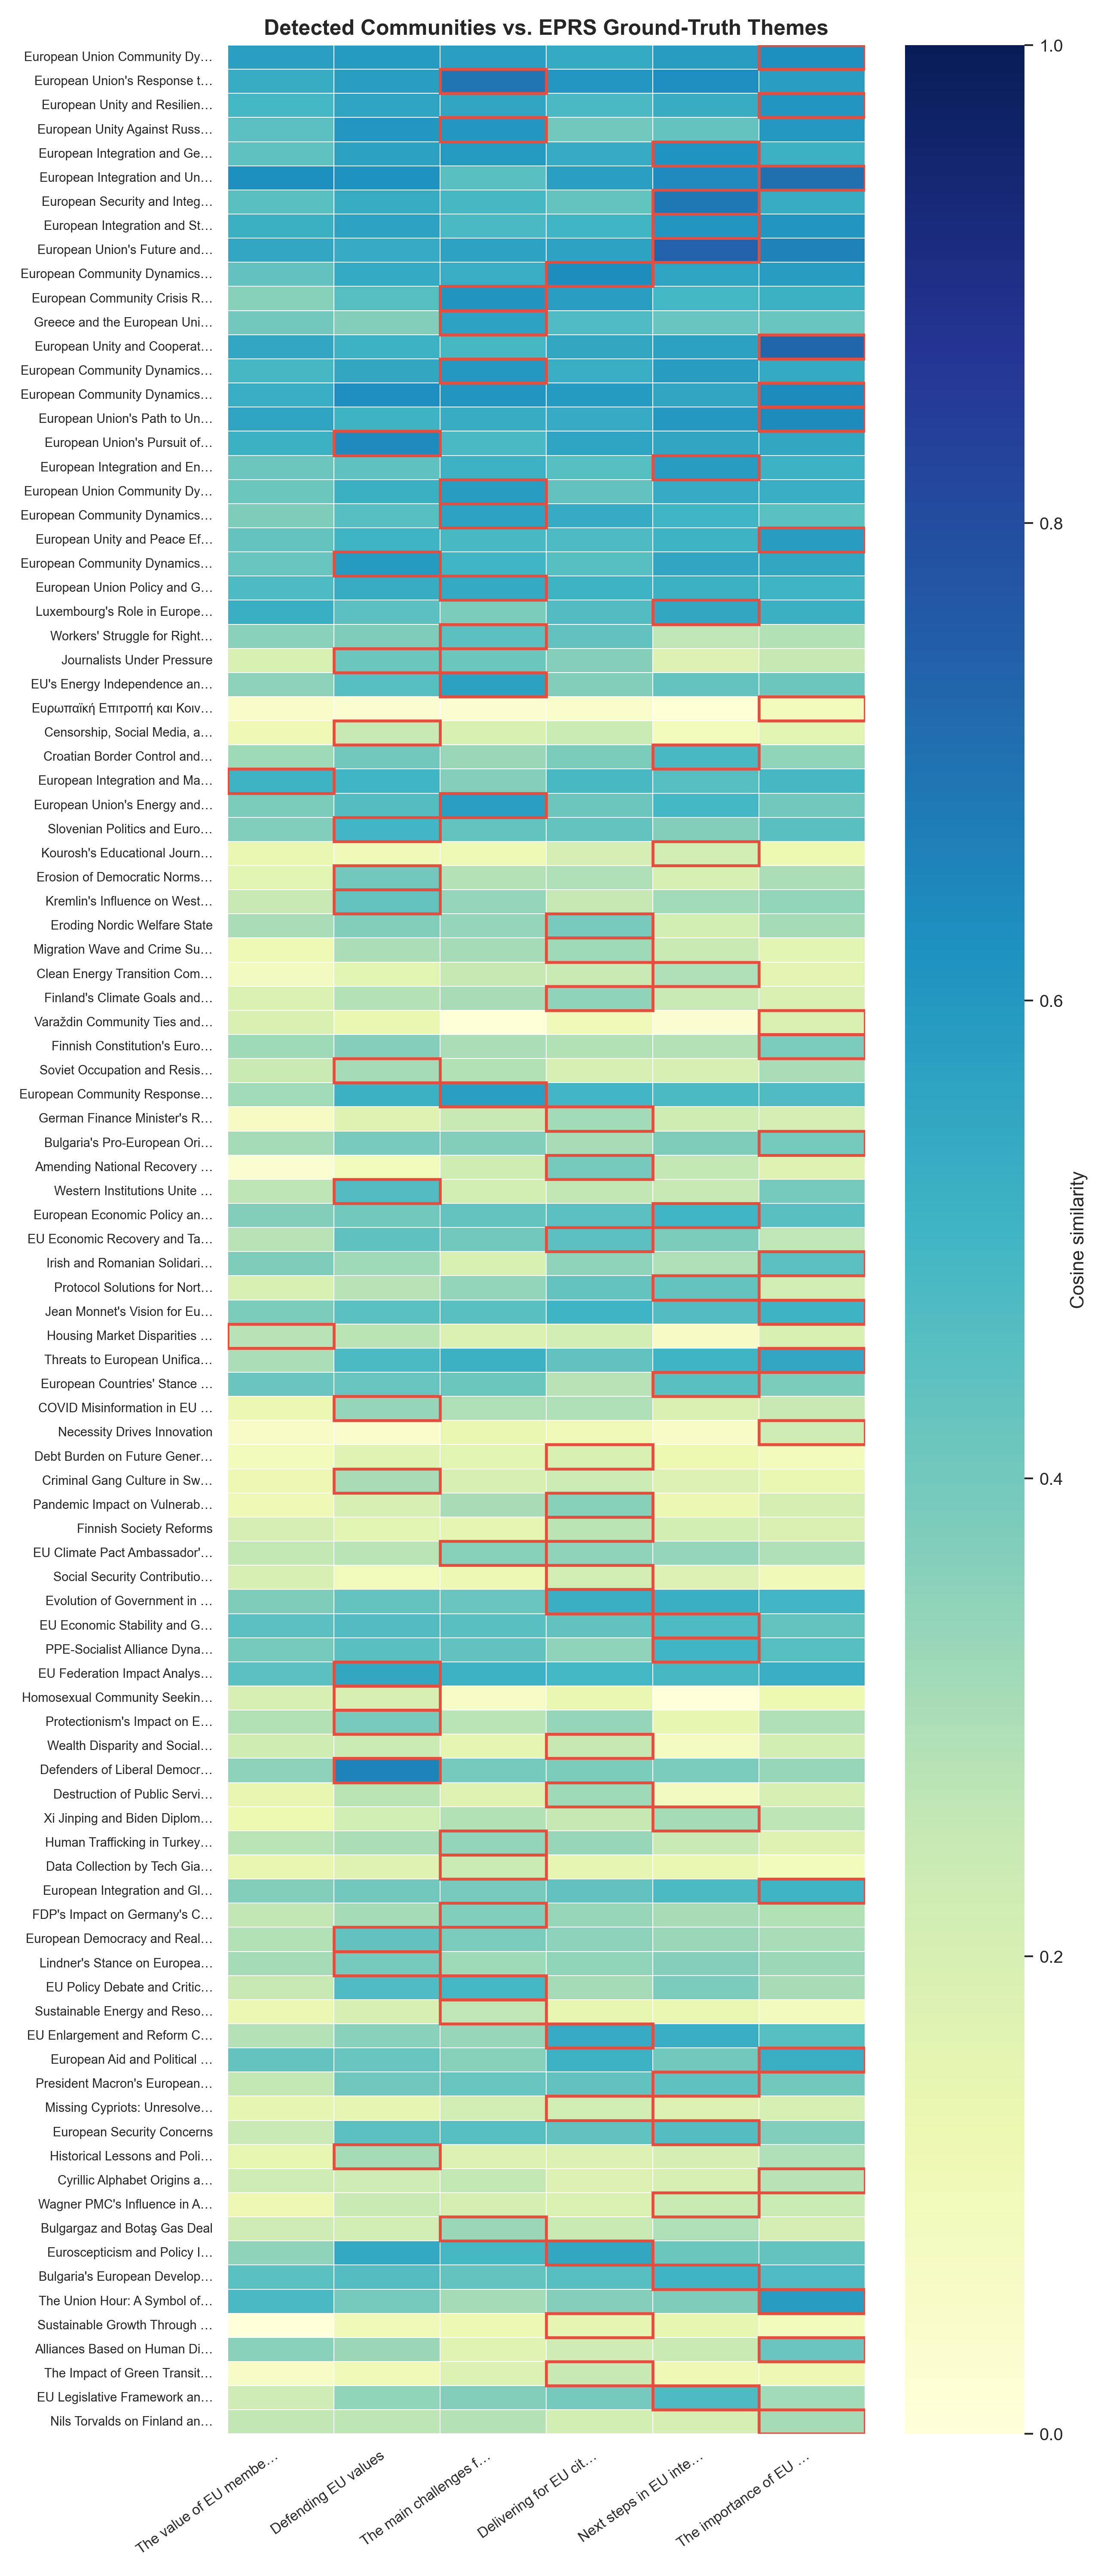
\includegraphics[width=0.92\textwidth]{figs/ground_truth_alignment_heatmap.png}
\caption{Cosine-similarity heatmap of community summaries against the six EPRS themes. Every theme finds at least one strong community match (coverage 100\%).}
\end{figure}

\subsection*{Drafted addition for \S4.3 (new paragraph before the qualitative discussion)}
\begin{draftbox}
Before turning to the qualitative mapping, the alignment can be stated quantitatively. Embedding each of the six recurring EPRS themes and matching it against all 99 community summaries by cosine similarity, \emph{every} EPRS theme finds a corresponding community (coverage $=100\%$), with a mean best-match similarity of 0.444. The strongest alignments are for EU unity (0.73), the next steps in integration (0.74), the EU's main challenges (0.69), and defending EU values (0.66). The number of communities that map to each theme is itself revealing: five of the six themes are the nearest theme for 18--21 communities apiece, confirming that these are the cross-cutting spine of the corpus, whereas ``the value of EU membership'' --- an abstract framing rather than a concrete subject --- is the nearest theme for only two. A mean similarity of 0.44 signals a thematic rather than a verbatim correspondence, which is appropriate: the pipeline recovers the EPRS's themes as regions of its topic landscape, not as identical labels.
\end{draftbox}

\clearpage
\section{Note on the discovered topics (\S4.1)}

The canonical run's 99 communities are dominated by one mega-community, TOPIC\_0 (``European Union Community Dynamics,'' \textbf{716 entities}), followed by a long tail of mid-sized communities (60--90 entities) and many minimal 3-entity communities (the median community size is 3). The three-tier structure described in the current \S4.1 --- dense core, policy-specific middle ring, niche periphery --- still holds, but the specific per-topic entity counts and titles differ from the earlier partial-graph draft and should be regenerated from \texttt{output/thesis\_outputs/topics.csv} before finalising. The community-size distribution is shown below.

\begin{figure}[h]
\centering
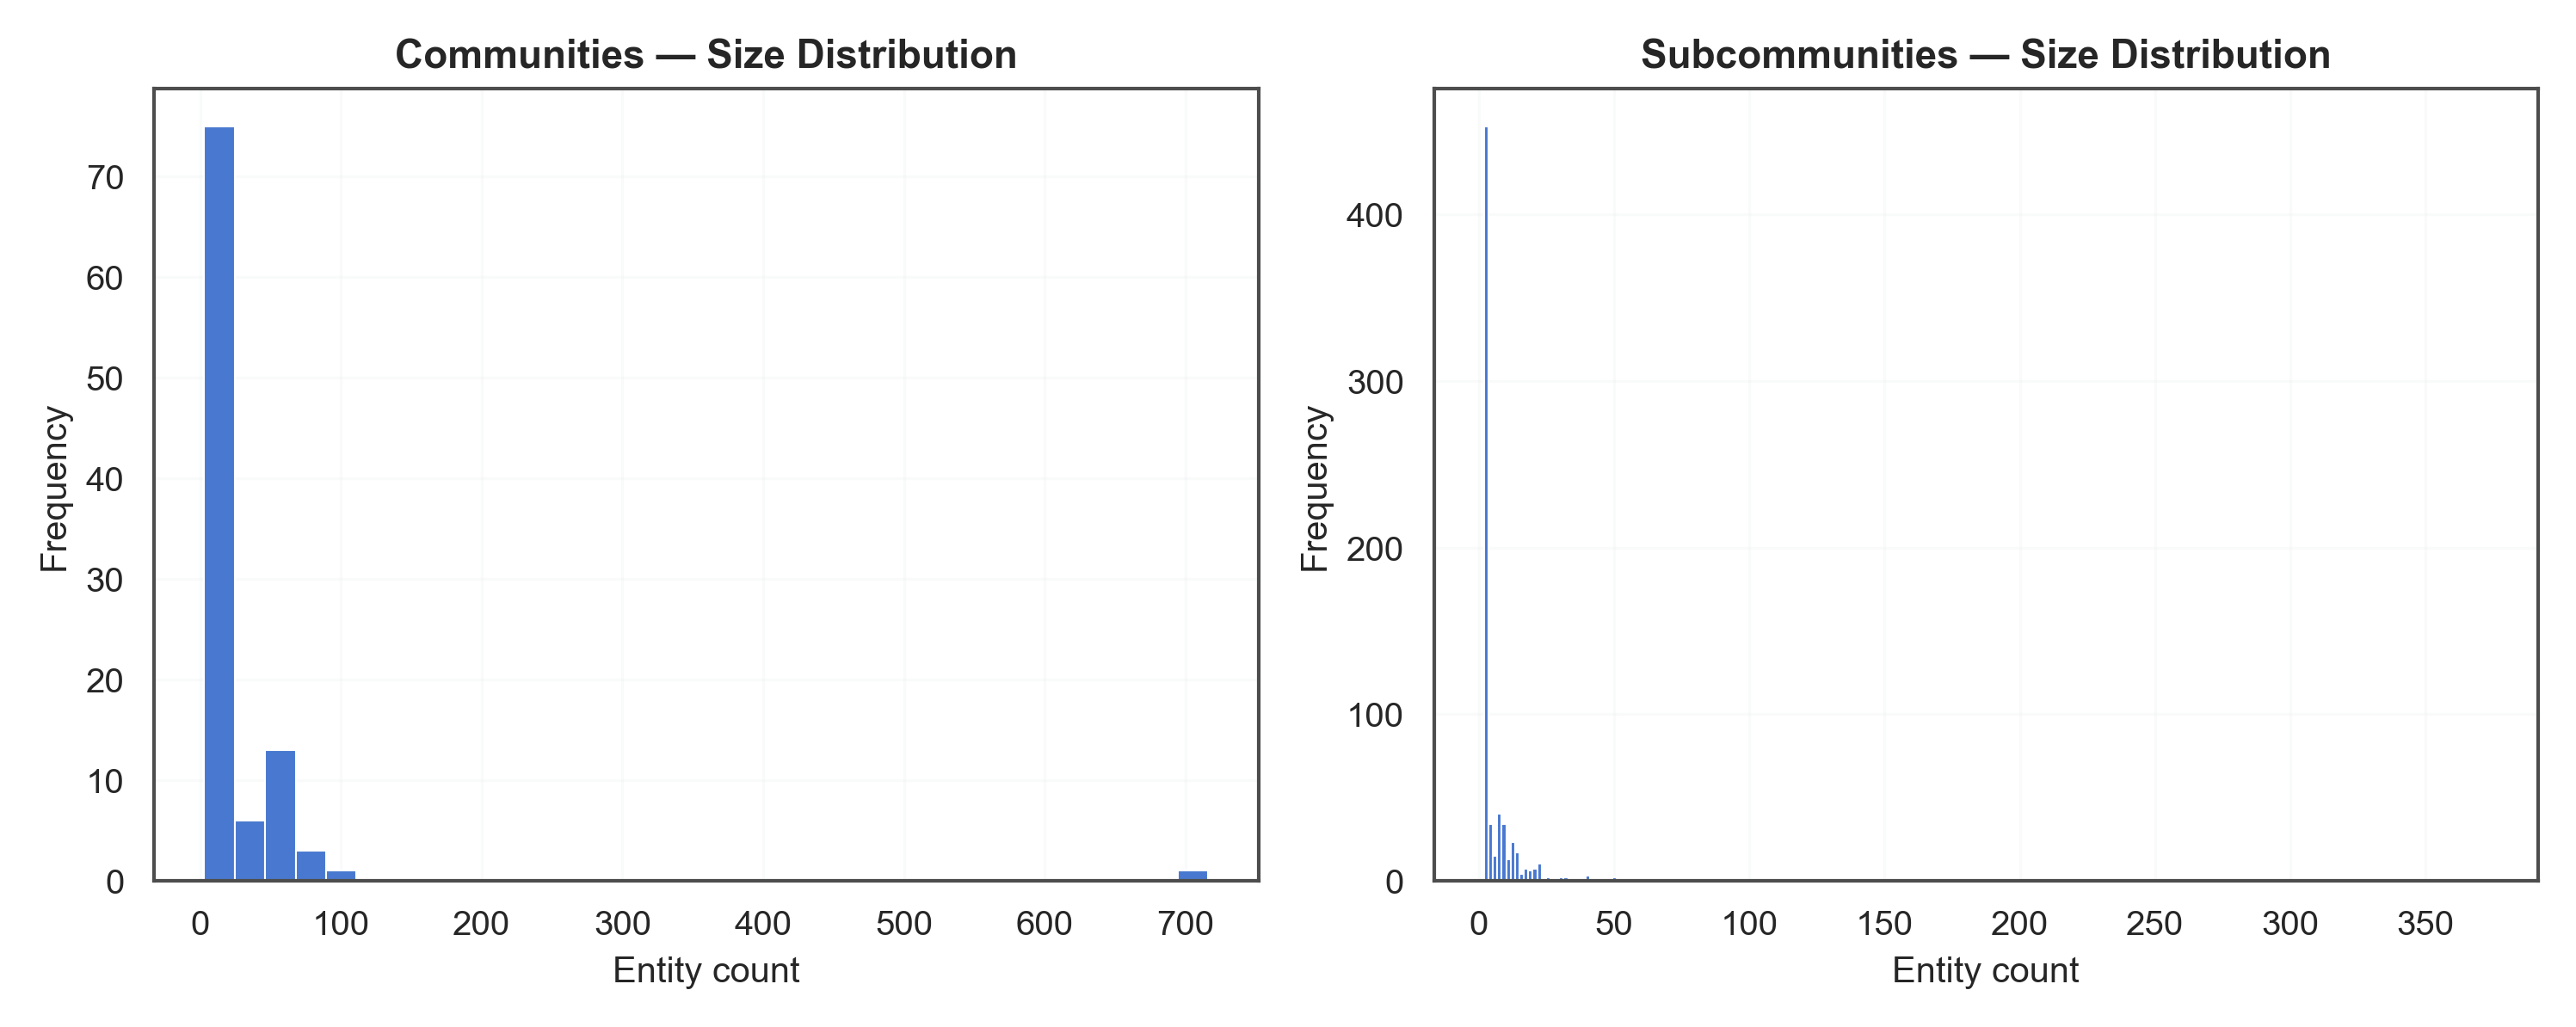
\includegraphics[width=0.8\textwidth]{figs/community_size_distribution.png}
\caption{Community-size distribution of the canonical run (99 communities; one 716-entity core, median size 3).}
\end{figure}

\begin{draftbox}
\textbf{Action item.} The qualitative topic walk-through in \S4.1 and the EPRS mapping table in \S4.3 of the current draft quote specific communities (e.g.\ ``TOPIC\_0: European Union in Crisis, 477 entities''). These come from the earlier 762-node graph and should be re-derived from the canonical run: TOPIC\_0 is now ``European Union Community Dynamics'' with 716 entities, and the mid-tier titles have shifted. The five findings above are method- and corpus-level and are already canonical; the per-topic narrative is the one remaining piece to refresh.
\end{draftbox}

\end{document}
